\documentclass[12pt]{article}
\usepackage[brazil]{babel}
\usepackage[utf8]{inputenc}
\usepackage[T1]{fontenc}
\usepackage{amsmath, amssymb}
\usepackage{geometry}
\usepackage{graphicx}
\usepackage{xcolor}

\definecolor{maincolor}{RGB}{0,100,50}
\usepackage{fancyhdr}
\definecolor{forestgreen}{RGB}{0,100,50}
\usepackage[most]{tcolorbox}
\newtcolorbox{block}[1]{%
  colback=green!5,
  colframe=maincolor,
  coltitle=white,
  title=#1,C
  fonttitle=\bfseries,
  boxrule=1.5pt,
  arc=3mm,
  left=6pt,
  right=6pt,
  top=6pt,
  bottom=6pt
}

\geometry{margin=2.5cm}
\pagestyle{fancy}
\fancyhf{}
\usepackage{tikz}
\usetikzlibrary{positioning,arrows.meta}
\renewcommand{\headrulewidth}{2pt}
\renewcommand{\footrulewidth}{2pt}

\renewcommand{\headrule}{\hbox to\headwidth{%
  \color{forestgreen}\leaders\hrule height \headrulewidth\hfill}}

\renewcommand{\footrule}{\hbox to\headwidth{%
  \color{forestgreen}\leaders\hrule height \footrulewidth\hfill}}

\setlength{\headheight}{32pt}

\fancyhead[L]{%
  
\includegraphics[height=1.2cm]{Universidade_de_Rio_Verde.jpg}
}

\fancyhead[R]{%
  \raggedleft
  \textcolor{forestgreen}{%
    \small
    \textbf{Lista de Exercícios — Programação Orientada a Objetos}\\
    Me.~Sergio Souza Novak\\
    \textit{Engenharia de Software}
  }
}

\fancyfoot[C]{%
  \textcolor{forestgreen}{\thepage}
}

\begin{document}

% ============================================================
\section*{1) Indústria 4.0 — Máquina CNC com Controle de Produção}
No contexto da Indústria 4.0, sistemas de manufatura inteligentes exigem controle automatizado de produção, monitoramento térmico em tempo real e manutenção preditiva baseada em horas de operação. Considere a modelagem da classe MaquinaCNC, responsável por representar uma máquina de usinagem com controle automatizado de funcionamento e segurança operacional.

\begin{center}
\begin{tikzpicture}[
class/.style={draw,rectangle,minimum width=7cm,align=left}
]

\node[class] {
\textbf{MaquinaCNC} \\
- modelo : String \\
- horasOperacao : double \\
- temperaturaAtual : double \\
- temperaturaMaxima : double \\
- ligada : boolean \\
- pecasProduzidas : int \\
+ ligar() : void \\
+ desligar() : void \\
+ produzir(qtd:int) : boolean \\
+ getTemperaturaAtual() : double \\
+ precisaManutencao() : boolean \\
- controlarTemperatura(qtd:int) : void \\
- verificarManutencao() : boolean
};

\end{tikzpicture}
\end{center}
\begin{figure}[h]
    \centering
    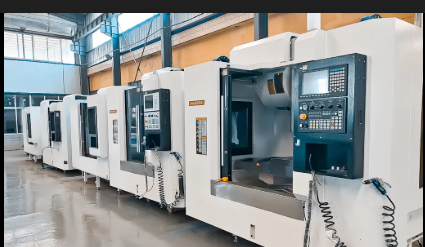
\includegraphics[width=0.65\textwidth]{usinagem.png}
    \caption{Máquina CNC em operação, ilustrando o processo de usinagem e controle térmico.}
\end{figure}
Considere a modelagem da classe \texttt{MaquinaCNC}, responsável por representar uma máquina de usinagem com controle automatizado de funcionamento e segurança operacional.

A classe deve encapsular os seguintes comportamentos:

\begin{itemize}
    \item Controle de estado da máquina (ligada/desligada).
    \item Produção de peças sob demanda.
    \item Monitoramento contínuo da temperatura de operação.
    \item Controle automático de superaquecimento.
    \item Verificação de necessidade de manutenção preventiva com base nas horas acumuladas de uso.
\end{itemize}

\subsection*{Requisitos Funcionais}

\begin{itemize}
    \item O método \texttt{ligar()} deve ativar a máquina.
    \item O método \texttt{desligar()} deve interromper completamente a operação.
    \item O método \texttt{produzir(qtd:int)} deve:
    \begin{itemize}
        \item Permitir produção apenas se a máquina estiver ligada.
        \item Atualizar o total de peças produzidas.
        \item Incrementar as horas de operação proporcionalmente à quantidade produzida.
        \item Retornar \texttt{true} se a produção ocorrer com sucesso e \texttt{false} caso contrário.
    \end{itemize}
    \item A temperatura deve aumentar proporcionalmente à produção realizada.
    \item Caso a temperatura ultrapasse o limite máximo permitido, a máquina deve ser desligada automaticamente por segurança.
    \item O método \texttt{getTemperaturaAtual()} deve retornar a temperatura corrente da máquina.
    \item O método \texttt{precisaManutencao()} deve indicar se a máquina ultrapassou o limite de horas de operação (por exemplo, 1000 horas).
    \item Métodos privados devem ser utilizados para:
    \begin{itemize}
        \item Controlar o aumento de temperatura.
        \item Verificar internamente a necessidade de manutenção.
    \end{itemize}
\end{itemize}

\subsection*{Regras de Negócio}

\begin{itemize}
    \item Não é permitido produzir com a máquina desligada.
    \item O controle térmico deve ser automático e transparente ao usuário da classe.
    \item A verificação de manutenção não pode ser manipulada externamente.
    \item Todos os atributos devem permanecer encapsulados (acesso restrito).
\end{itemize}

% ============================================================
\section*{2) Siderurgia — Alto Forno com Controle Termodinâmico}
Considere a modelagem da classe \texttt{AltoForno}, que representa um equipamento industrial utilizado para produção de metal em uma siderúrgica.

\begin{center}
\begin{tikzpicture}[
class/.style={draw,rectangle,minimum width=7cm,align=left}
]

\node[class] {
\textbf{AltoForno} \\
- temperaturaInterna : double \\
- temperaturaMinimaOperacao : double \\
- temperaturaMaximaOperacao : double \\
- volumeMetalProduzido : double \\
- ativo : boolean \\
+ iniciarForno() : void \\
+ desligarForno() : void \\
+ injetarCombustivel(qtd:double) : double \\
+ produzirMetal() : double \\
+ estaAtivo() : boolean \\
- verificarFaixaTermica() : boolean \\
- controleSeguranca() : void
};

\end{tikzpicture}
\end{center}

O alto-forno opera em altas temperaturas e precisa estar ativo para produzir metal. O controle de temperatura é essencial para garantir que a produção ocorra corretamente.

\begin{figure}[h]
    \centering
    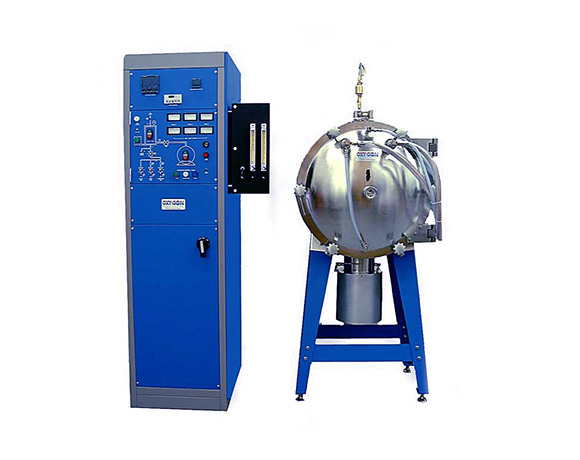
\includegraphics[width=0.65\textwidth]{fornoaltovacuo_580x460.jpg}
    \caption{Forno de alto-forno em operação, ilustrando o processo de produção de metal e controle termodinâmico.}
\end{figure}
\subsection*{Requisitos}

\begin{itemize}
    \item O método \texttt{iniciarForno()} deve ativar o forno.
    \item O método \texttt{desligarForno()} deve desativar o forno.
    \item O método \texttt{estaAtivo()} deve retornar se o forno está ligado ou desligado.
    \item O método \texttt{injetarCombustivel(qtd:double)} deve aumentar a temperatura interna e retornar o novo valor da temperatura.
    \item O método \texttt{produzirMetal()} deve:
    \begin{itemize}
        \item Produzir metal apenas se o forno estiver ativo.
        \item Produzir metal apenas se a temperatura estiver dentro da faixa mínima e máxima de operação.
        \item Retornar a quantidade produzida na operação.
    \end{itemize}
\end{itemize}

\subsection*{Regras de Negócio}

\begin{itemize}
    \item Não é permitido produzir metal com o forno desligado.
    \item Não é permitido produzir metal se a temperatura estiver abaixo do mínimo ou acima do máximo definido.
    \item Caso a temperatura ultrapasse o limite máximo, o forno deve ser desligado automaticamente.
    \item Todos os atributos devem permanecer privados.
\end{itemize}

% % ============================================================
% \section*{3) Logística Portuária — Sistema de Containers Inteligentes}

% \begin{center}
% \begin{tikzpicture}[
% class/.style={draw,rectangle,minimum width=7cm,align=left}
% ]

% \node[class] {
% \textbf{ContainerRefrigerado} \\
% - codigo : String \\
% - pesoAtual : double \\
% - pesoMaximo : double \\
% - temperaturaInterna : double \\
% - temperaturaIdeal : double \\
% - ativo : boolean \\
% + ativarRefrigeracao() : void \\
% + desativarRefrigeracao() : void \\
% + adicionarCarga(peso:double) : boolean \\
% + monitorarTemperatura() : double \\
% + estaAtivo() : boolean \\
% - ajustarTemperatura() : void \\
% - verificarPeso() : boolean
% };

% \end{tikzpicture}
% \end{center}

% \section*{5) Agronegócio — Sistema Inteligente de Irrigação}

% \begin{center}
% \begin{tikzpicture}[
% class/.style={draw,rectangle,minimum width=6.5cm,align=left}
% ]

% \node[class] (sensor) {
% \textbf{SensorSolo} \\
% - umidadeAtual : double \\
% + atualizarLeitura(valor:double) : void \\
% + getUmidade() : double \\
% + estaSeco(limite:double) : boolean
% };

% \node[class, right=4cm of sensor] (controlador) {
% \textbf{ControladorIrrigacao} \\
% - sensor : SensorSolo \\
% - irrigando : boolean \\
% - limiteMinimoUmidade : double \\
% + verificarIrrigacao() : boolean \\
% + estaIrrigando() : boolean \\
% - iniciarIrrigacao() : void \\
% - pararIrrigacao() : void 
% };

% \draw[-{Latex}] (controlador) -- node[above]{1} (sensor);

% \end{tikzpicture}
% \end{center}

% ============================================================
\end{document} 